    \subsection{Missing Values}
        Non applicable, undisclosed or generated by errors information, we must deal with them (and we see some techniques).\\
        Some of the techniques can directly deal with missing values while others instead need some additional preprocessing.\\
        Dealing with missing values:
        \begin{itemize}
            \item \textbf{Replace:} with known values like the mean or median
            \item \textbf{Delete:} if the feature is uncorrelated with the label, we can delete it
            \item \textbf{Keep:} some missing values can be meaningful and may have a relation with frauds, so they must be considered as a separate category
        \end{itemize}
        Perform a statistical test to understand if the missing value is correlated or not with the target label, this will impact the choice made to cope with these values.
        \subsubsection{Example:}
            \begin{figure}[ht!]
                \centering
                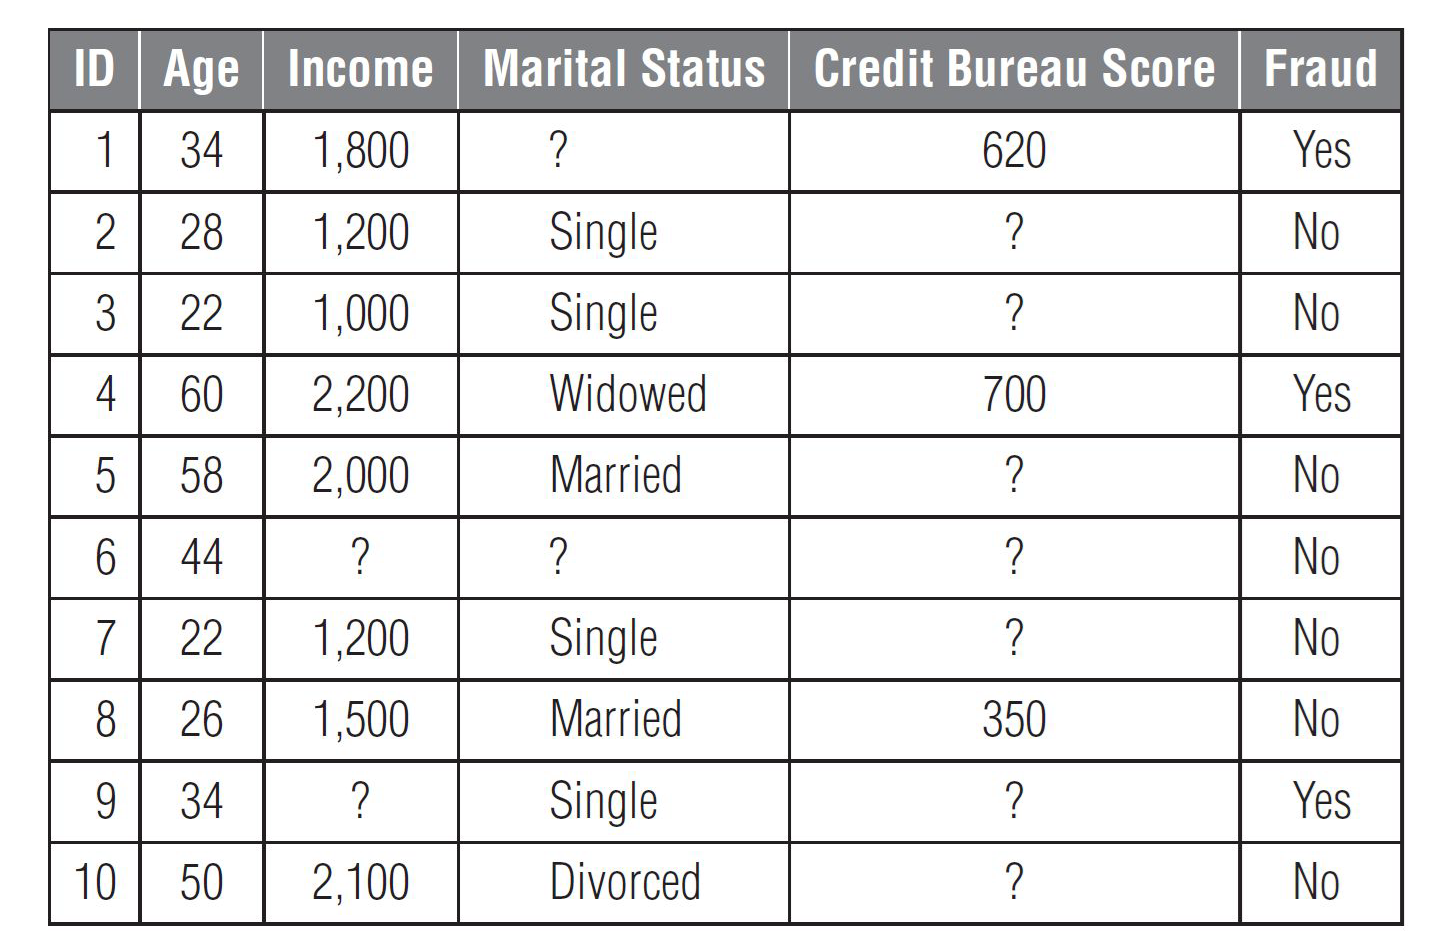
\includegraphics[width=0.6\linewidth]{lecture_13/example.png}
            \end{figure}
            \begin{itemize}
                \item Here for example is possible to delete row 6 because of the number of missing values.
                \item Many missing values are present also in the credit bureau score, but in this case we see that the rows where it is inserted are labeled as frauds, it is better to keep the missing values or to replace them with an average or something.
                \item Marital status for entry 1 will be missing: if we use our knowledge to put a value, we risk to introduce bias, an alternative solution can be to use the mode of the dataset.
            \end{itemize}
    \subsection{Outliers}
        Outliers are extreme observations that are very dissimilar from the rest of the population.
        \begin{itemize}
            \item Valid: boss salary is \$ 1,000,000
            \item Invalid: age is 300 
        \end{itemize}
        In this specific part of the processing step we want to identify the outliers that may influence too much our model, we call:
        \begin{itemize}
            \item \textbf{Univariate Outliers} the ones which outly in one dimension
            \item \textbf{Multivariate Outliers} the ones which outly in multiple dimensions
        \end{itemize}
        \subsubsection{Univariate Outlier Detection and Treatment}
            Minimum and maximum values for each of the data elements.
            \begin{itemize}
                \item Graphical Tools:
                \begin{itemize}
                    \item Histograms (grafico a torre): check for values less frequent from the average, if included they may introduce bias
                    \item Box Plot: It is a plot which represents three key quartiles of the data to find values far from them 
                \end{itemize}
                \item Z-scores: measures how many standard deviations and observation lies away from the mean, computes the difference of the sample from the mean, and then divides for the std deviation
            \end{itemize}
        \subsubsection{Multivariate Outlier Detection and Treatment}
            \begin{itemize}
                \item Fit regression lines and inspect the observations with large errors 
                \item Make some statistical test to understand what to do with them
            \end{itemize}
        \subsubsection{How to deal with outliers}
            Various schemes:
            \begin{itemize}
                \item Invalid observations can be treated as missing values 
                \item Valid observation can be capped to a maximum or minimum value
            \end{itemize}
        \subsubsection{Expert-based outlier detection}
            Not all invalid values are outlying and may go unnoticed if not explicitly looked into.\\
            Apply some rules based on expert knowledge to data to check and alert for issues, as existing relations between the different variables
            \paragraph*{Example:}
                \begin{itemize}
                    \item Birthdate: 1/01/1980
                    \item Category: Child
                \end{itemize}
                We don't know which of the two is the invalid value, but we know that the pair is. Both values are not outlying and therefore explicit precautions must be taken to notice.
    \subsection{Standardizing Data}
        \subsubsection{Euclidean vs Manhattan distance}
            \begin{figure}[ht!]
                \centering
                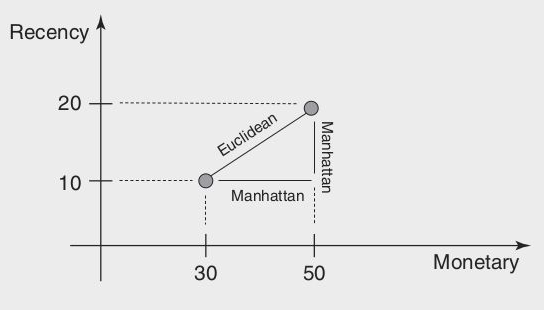
\includegraphics[width=0.6\linewidth]{lecture_13/distances.png}
            \end{figure}
            \begin{itemize}
                \item Euclidean: $$\sqrt{(1500-1000)^2 + (10-5)^2} = 500$$
                \item Manhattan: $$ |1500-1000| + |10-5| = 505$$
            \end{itemize}
            \textbf{Warning:} the distance between monetary is more determining than the one for recency, there is the need to standardize.
        \subsubsection{Standardization}
            Means to scale variables to a similar range, multiple techniques are available:
            \begin{itemize}
                \item \textbf{Min/Max standardization:} impose a new max and a new min and scale accordingly
                \item \textbf{Z-score standardization:} calculate the z-scores
                \item \textbf{Decimal scaling}
            \end{itemize}
    \subsection{Categorization}
        For categorical variables, it is needed to reduce the number of categories.\\
        Basic methods:
        \begin{itemize}
            \item \textbf{Equal interval binning:} create bins with the same range
            \item \textbf{Equal frequency binning:} create bins with the same number of observations
            \item \textbf{Chi-squared analysis}
            \item \textbf{Pivot table}
        \end{itemize}
    \subsection{Variable Selection}
        Typically, only few variables contribute to the prediction. We need to select only the helpful ones.\\
        Usually, in fraud detection domain, the number of variables is in the range of 10-15, how do we find them?
        \subsubsection{Filters}
            It is a selection mechanism based on statistical tests. Allow a quick screening of which variables should be retained for further analysis. They allow reduction in the number of dimensions of the data set early in the analysis.
            Drawbacks:
            \begin{itemize}
                \item They do not consider correlation betwen dimensions
            \end{itemize}
        \subsubsection{Principal Component Analysis}
            Dimension reduction by forming new linearly independent variables, which are linear combinations of the original set, which have the property to better describe the distribution.\\
            The new variables are called principal components. The variance contained in the original data can be summarized by a limited number of principal components. Left out the ones which account for a very small fraction of variance.
            Limitations:
            \begin{itemize}
                \item \textbf{Reduced interpretability:} a transaction may be labeled as fraudulent whithout us knowing why because of the strange form of features.
            \end{itemize}
\section{Unsupervised Learning for Fraud Detection}
    Unsupervised learning aims at finding anomalous behavior deviating from the \textbf{norm}.\\
    The challenge is to find a way to correctly model the norm, like the behavior of the average customer at a snapshot in time or the average behavior of a given customer across a time period.
    \subsection{Unsupervised learning = anomaly detection}
        It aims at finding anomalies, useful when:
        \begin{itemize}
            \item Organizations are starting doing fraud detection 
            \item No labeled historical dataset available 
            \item Fraudsters are continously adapting
        \end{itemize}
    \subsection{Unsupervised Learning Challenge}
        \textbf{Define the average behavior or norm:} 
        \begin{itemize}
            \item it depends on the application field
            \item Boundary between norm and outliers is not clear-cut (fraudsters try to blend into norm)
            \item The norm may change overtime
        \end{itemize}
        Anomalies do not necessarily represent frauds, unsupervised learning for fraud detection requires extensive validation of the identified suspicious observations
    \subsection{Basic tasks to find anomalies}
        \begin{itemize}
            \item \textbf{Graphical outlier detection:} find outliers with histograms or box plots for the one-dimensional, with scatter plots for the multi-dimensional
            \begin{itemize}
                \item Disadvantages: less formal and limited to few dimensions, requires active end-user involvement, very difficult to perform for a large dimensional dataset
            \end{itemize}
            \item \textbf{Statistical outlier detection:}
            \begin{itemize}
                \item Use z-score: if the z-score is bigger than 3 consider outliers 
                \item Fit a distribution: outliers are the observations with small values for the probability density distribution 
                \item \textbf{Break Point Analysis}
                \item \textbf{Peer Group Analysis}
            \end{itemize}
        \end{itemize}
        \subsubsection{Break Point Analysis}
        \subsubsection{Peer Group Analysis}
        \subsubsection{Example: Credit card fraud}
        \subsubsection{Break Point vs Peer Group analysis}
\iffalse

    Statistical outlier detection 
        z-score 
        fit a distribution 
        break point analysis 
        peer group analysis

        Break point analysis
            intra-account method 
                ha detto delle cose 
                detect a breakpoint in your ds and compare the distributions before and after this breakpoint 
                breakpoint is a sudden change in an account behavior 
                example slide 71
                    compare the distribution of the old model wrt new model's 
                    t-score (slide 72)
        
        peer group analysis 
            inter-account fraud detection method 
            Peer group is a group of accounts which have similar behavior to the target account 
            when an account's behavior deviates substantially from it's peers then an anomaly is signaled 
                1- identify the peer group, using prior, statistical way(similarity metrics)
                    define the number of peers (too small) -> noise sensitive 
                                                (too big) -> insensitive to local
                poi ha detto cose? Chi lo sa? 13:39 

            CC fraud example 
                weekly amount time series 
                    verify whether the amount spent at timestep n is anomalous 
                    c'è il disegno 
                    consider the peer group and see if the amount spent is anomalous wrt peer group 

        These techniques are the basis for existing unsup. learning techniques.
            What are the advantages and disadvantages of peer-group/break-point analysis 
                if we consider months from january to november, everything performed in december can be cosnidered anomalous (Christmas)
                for sure the main disadvantage is that they have issues with seasonality
                What can we do to limit the problem of seasonality?
                    peers will behave similarly during christmas, so it depends on the objective of your fraud detection system
                    if it might be efficient enough you can think to combine the two approaches 
                    ha aggiunto cose (13:47)
    Clustering (ultimi 2 minuti)
\fi